% 
% topic Template for ME3050 -  Dynamics Modeling and Controls - Tennessee Technological University
%
% Spring 2020 - Summer 2020
% Tristan Hill, May 07, 2020
% Dyanmics Review - Topic 2 - Units and Conversions
%

\documentclass{beamer}                         % for presentation (has nav buttons at bottom)
%\documentclass[handout]{beamer}  % for handout 
\usepackage{beamerthemesplit}
\usepackage{amsmath}
\usepackage{listings}
\usepackage{multicol}

\beamertemplateballitem

\definecolor{TTUpurple}{rgb}{0.3098, 0.1607, 0.5176} % TTU Purple (primary)
\definecolor{TTUgold}{rgb}{1.0000, 0.8666, 0.0000} % TTU Gold (primary)

\setbeamercolor{palette primary}{bg=TTUpurple,fg=TTUgold}
\setbeamercolor{palette secondary}{bg=black,fg=TTUgold}
\setbeamercolor{palette tertiary}{bg=black,fg=TTUpurple}
\setbeamercolor{palette quaternary}{bg=TTUgold,fg=black}
\setbeamercolor{structure}{fg=TTUpurple} % itemize, enumerate, etc
\setbeamercolor{section in toc}{fg=TTUpurple} % TOC sections

%\usefonttheme{professionalfonts}



\newcommand{\Lagr}{\mathcal{L}} % lagrangian

\newcommand{\vspccc}{\vspace{6mm}\\} % large vertical space
\newcommand{\vspcc}{\vspace{4mm}\\}   % medium vertical space
\newcommand{\vspc}{\vspace{2mm}\\}     % small vertical space

\newcommand{\hspcccc}{\hspace{10mm}} % large horizontal space
\newcommand{\hspccc}{\hspace{6mm}} % large horizontal space
\newcommand{\hspcc}{\hspace{4mm}}   % medium horizontal space
\newcommand{\hspc}{\hspace{2mm}}     % small horizontal space


\author{ME3050 - Dynamics Modeling and Controls} % original formatting from Mike Renfro, September 21, 2004

\newcommand{\TNUM}{2\hspace{2mm}} % topic Number 
\newcommand{\topictitle}{Topic \TNUM - Units and Conversions} % first line of title (used by beamer)
\newcommand{\sectiontitle}{Dynamics Review }% second line of the title of this presentation (used by TWH)

\title{\sectiontitle - Topic \TNUM}

\date{May 29, 2020}

\begin{document}

\lstset{language=MATLAB,basicstyle=\ttfamily\small,showstringspaces=false}

\frame{\titlepage \center\textbf{\topictitle}\vspace{5mm}\\}

% Section 0: Outline


\frame{

\large \textbf{\topictitle} \vspace{3mm}\\

%Topics : \vspace{3mm}\\ % ' topics' are beamer 'sections' - TWH

\begin{itemize}	
	\item Standard Units\vspace{3mm}\\ % Section 1
	\item Unit Conversions\vspace{3mm}\\% Section 2
	\item Frequency and Circular Frequency \vspace{3mm}\\ %Section 3
	\item Famous Example - Units Matter !!!\vspace{3mm}\\ % Section 4
\end{itemize}
}

% Section 1
\section{Standard Units}

\frame{
\frametitle{Standard Units}

\renewcommand{\arraystretch}{1.2}
\begin{tabular}{|c|c|c|c|c|} \hline
\textbf{Quantity}&\textbf{Unit(SI)} &\textbf{ Symbol(SI)}&\textbf{Unit(US)}&\textbf{Symbol(US)}\\ \hline
time&second&(s)&second&(sec)\\ \hline
length&meter&(m)&foot&(ft)\\ \hline
force&newton&(N)&pound&(lb)\\ \hline
mass&kilogram&(kg)&slug&(?) \\\hline
energy&joule&(J)&foot-pound&(ft-lb)\\ \hline
power&watt&(W)&?&(ft-lb/sec)\\ \hline
temp.&degrees&$^\circ C$, $^\circ K$&degrees&$^\circ F$, $^\circ R$ \\ \hline
\end{tabular}

\vspace{3mm}When possible work in the {\it base} units. SI is prefered but in the US we must know both systems.

}

% Section 2
\section{Unit Conversions}

\frame{
\frametitle{Unit Conversions}

If you are unsure about the units, WRITE THEM OUT!

I prefer to write them out as fractions and cancel. \vspc

\underline{Example}: Find exactly how many seconds are in 3 days. \vspcc

\scalebox{1.0}{$3$ Days $=$} 


}

% Section 3
\section{Frequency and Circular Frequency}

\frame{
\frametitle{Frequency and Circular Frequency}

\begin{multicols}{2}

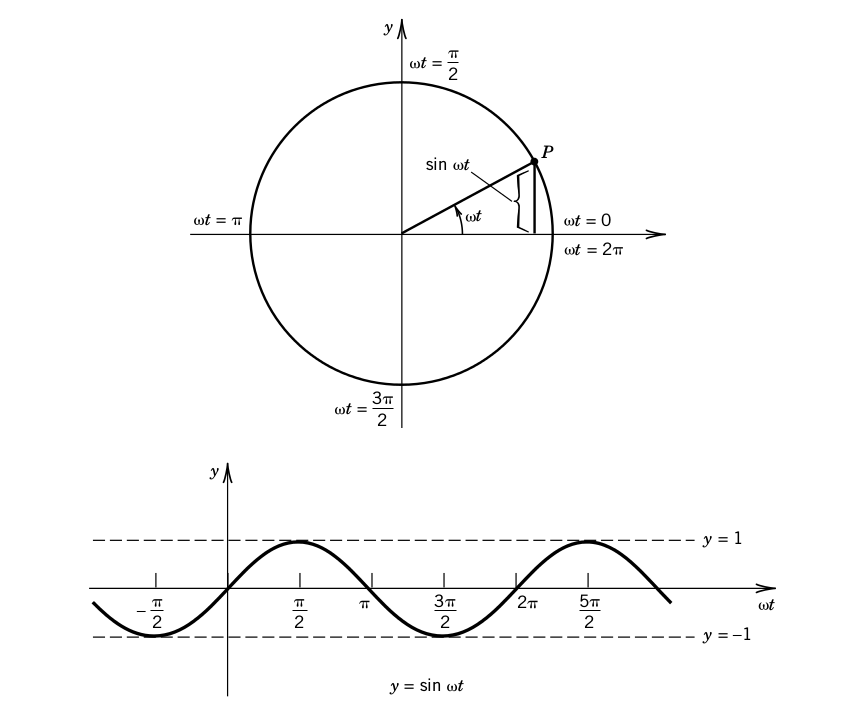
\includegraphics[scale=.35]{circular_frequency.png}

Frequency ($Hz$) and circular-frequency ($\frac{rad}{s}$) are both commonly used.  \vspace{15mm}

You can easily convert from one to the other.
\end{multicols}

}

% Section 4
\section{Famous Example - Units Matter !!!}

\frame{
\frametitle{Famous Example - Units Matter !!!}

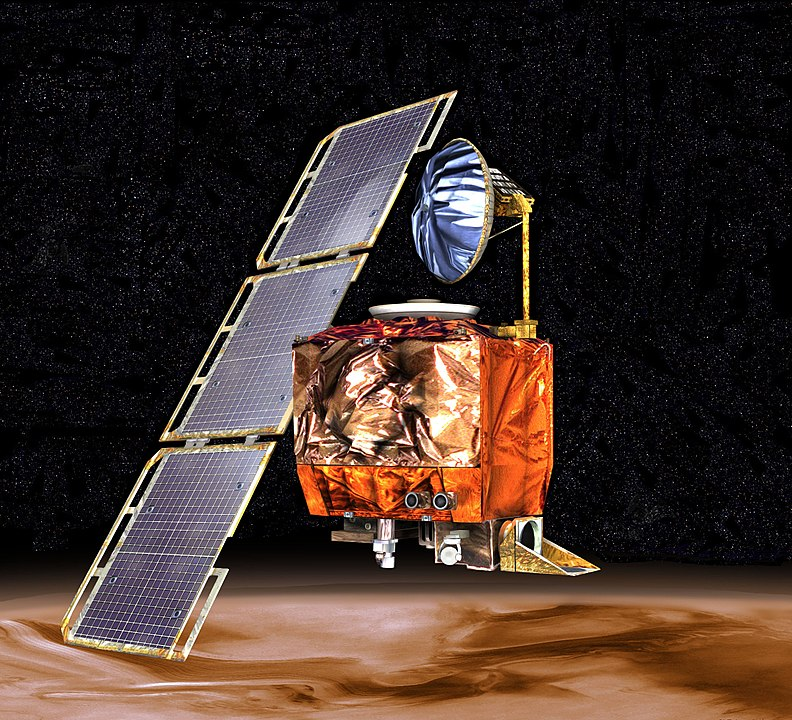
\includegraphics[scale=.1]{mars_orbiter.jpg}
The Mars Climate Orbiter (formerly the Mars Surveyor '98 Orbiter) was a 638-kilogram (1,407 lb)[1] robotic space probe launched by NASA on December 11, 1998 to study the Martian climate, Martian atmosphere, and surface changes and to act as the communications relay in the Mars Surveyor '98 program for Mars Polar Lander. {\tiny \href{https://en.wikipedia.org/wiki/Mars_Climate_Orbiter}{Full Story: Wikipedia} }

}



\end{document}

	





